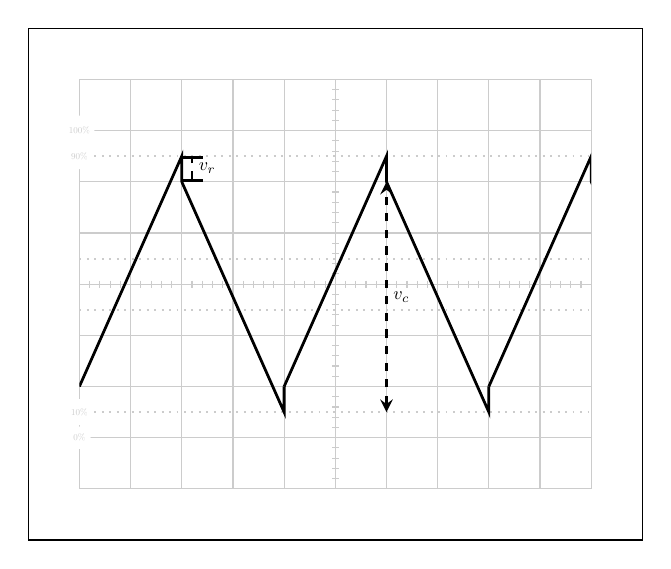
\begin{tikzpicture}[scale=0.65,every node/.style={transform shape}]
\def\res{0.5};%EscalaTemporal señal 1
\def\ind{1};%EscalaTemporal señal 2
\def\scalVa{1};%EscalaVertical señal 1
\def\frec{5};%EscalaVertical señal 2
\def\offseta{0};%Nivel de offset de la señal señal 1
\def\offsetb{};%Nivel de offset de la señal señal 2

%Lineas intermedias grilla
\foreach \x in {-5,-4.8,...,4.8,5}{
    \draw[gray!40,thin,shift={(\x,0)}] (0pt,2pt) -- (0pt,-2pt);
}
\foreach \y in {-4,-3.8,...,3.8,4}{
    \draw[gray!40,thin,shift={(0,\y)}] (2pt,0pt) -- (-2pt,0pt);
}
\foreach \a [evaluate={\y=\a*0.5}] in {-5,-1,1,5}{
    \draw[gray!40,line width=0.7pt,dotted] (-5,\y) -- (5,\y);
}

%Grilla
\draw[thin,gray!40] (-5,-4) grid (5,4);
\node[fill=white,text=gray!40,circle,scale=0.5] at (-5,3) {$100\%$};
\node[fill=white,text=gray!40,circle,scale=0.5] at (-5,2.5) {$90\%$};
\node[fill=white,text=gray!40,circle,scale=0.5] at (-5,-2.5) {$10\%$};
\node[fill=white,text=gray!40,circle,scale=0.5] at (-5,-3) {$0\%$};
\draw[black] (-6,-5) rectangle(6,5);

%Señal 1
\clip (-5,-4) rectangle (5,4);
\foreach [evaluate={\a=\c+2}] \c in{-5,-1,3}{
    \draw[line width=1pt](\c,-2)--(\a,2.5)--(\a,2){};
    \draw[line width=1pt](\a,2)--(\a+2,-2.5)--(\a+2,-2){};
}
\draw[line width=1pt,dashed,stealth-stealth](1,-2.5)--(1,2) node[midway,right]{$v_c$};
\draw[line width=1pt,dashed,stealth-stealth,|-|](-2.8,2)--(-2.8,2.5)node[anchor=north west]{$v_r$};
\end{tikzpicture}